\chapter{Multi-tenancy}
\index{Multi-tenant}
This chapter aims to introduce the concepts and ideas surrounding multi-tenancy and explain why it is relevant or even important to current cloud computing \index{Cloud Computing} practices.

\section{The Cloud}

Cloud computing is commonly defined as a form of computing where computing resources are shared in contrast to having local dedicated resources to run applications or services \cite{webopedia}. Walker \cite{GraceWalker} further defines cloud computing as a solution that delivers IT as a service by using computers to work together and applications to utilize these collective computing power as a single system.
 
The creation of public clouds, which offer cloud solutions to the general public, has provided anyone with almost unlimited resources and scalability. Large numbers of companies are shifting to using public clouds instead of maintaining their own data centres. The large cost advantages resulting from using the public cloud is the primary factor fuelling this shift, allowing stronger competition between companies of all sizes. Although cloud computing is not a new technology, but simply a way that computing resources are delivered (much akin to historic mainframes). It is a major paradigm shift in the way information and services are provided \cite{GraceWalker}. All of this has created a need for radical redefinition of our current computer architectures, software, tools, persistence mechanism and design patterns \cite{GraceWalker}. Applications design should be continuously aware of the cloud computing layers including Infrastructure as a Service (IaaS), \index{Infrastructure as a Service (IaaS)} Platform as a Service (PaaS)\index{Platform as a Service (PaaS)} and Software as a Service (SaaS), \index{Software as a Service (SaaS)} and be designed to natively support deployment and management through them. Bill Wilder \cite{webopedia} defines applications as cloud-native \index{Cloud-native} if they are architected to take advantage of proven engineering practices that utilize cloud platform services to cost efficiently and automatically allocate resources allowing horizontal scaling, handle hardware failures without downtime and minimize network latency, all automatically.


\section{What is Multi-tenancy?}

Krebs defines multi-tenancy as an approach to share a single application instance between multiple tenants by providing each tenant a dedicated share of the instance which is isolated from other shares with regards to performance and data privacy \cite{Krebs2012}.
Wilder \cite{Wilder2012-so} defines multi-tenancy as a system shared by tenants, usually operated by a single company. Furthermore, Bezemer goes on to extend these definitions by stating that multi-tenant applications should allow tenants to configure the application to meet their specific needs as if it was running on a completely dedicated environment\cite{Bezemer:2010:MSA:1862372.1862393}. While these definitions do thoroughly express the basic principle of multi-tenancy, in a broader sense, it does not provide a strong view from which such systems can be architected. It is therefore that I attempt to provide a more concise, amalgamated and personal definition of multi-tenancy in respect to this research as follow:
\\
\begin{fancyquotes}
Multi-tenancy is a [software] architecture principle which dictates the sharing of physical computing resources by groupings of tenants by utilizing a single application instance that is limitlessly, horizontally scalable, while logically isolating each one of its tenants.
\end{fancyquotes}
\\
This definition, however leaves to question the exact meaning of a tenant. One definition of a tenant is a grouping of customers that are a closed, charged and handled together \cite{Krebs2012}. Bezemer suggests that these groupings are stakeholders in an organization  \cite{Bezemer:2010:MSA:1862372.1862393} while Wilder defines tenants as specific groupings of users that have their own respective employees or customers that can access the system while sharing a common view \cite{Wilder2012-so}.
Some of the key aspects of multi-tenant applications has been summarized as follow \cite{Bezemer:2010:MSA:1862372.1862393}
\begin{enumerate}
\item The application should be able to share hardware resources
\item The application should be highly configurable
\item  The application should use a single instance and in pure multi-tenant solutions, even a single database instance should be used
\end{enumerate}

\section{An Analogy for Multi-tenancy}

A common analogy for multi-tenancy can be made by comparing multi-tenant software systems with an apartment block. Software tenants are considered a closed group of customers that are handled together and usually share a common view of the system \cite{Krebs2012} \cite{Wilder2012-so}. This means that like in the apartment block, tenants are a grouping of customers (people/families/businesses) using the system (living in an apartment). In such an apartment block, a tenant is an owner of their own respective apartment. Each tenant lives and operates within their apartment independently of other tenants. The tenant could also have other people living or working in his apartment while being completely isolated from the apartment block and other tenants as a whole. Although each tenant lives and acts as if they own the entirety of their apartment block, they are actually sharing resources with all the other tenants including electricity, heating and property space. In contrast classical software systems represent a house, where only a single-tenant lives and all resources are consumed and used by that tenant. Building a house for each family (grouping of customers or tenant) is extremely expensive and in many cases simply not feasible. This is especially true since everyone wants to pay the minimum amount of money for a place to live.

\section{Multi-tenant vs. Single-tenant}

The difference between multi-tenant and single-tenant systems can clearly be outlined as in figure \ref{fig:multi-vs-single}. This diagram shows how an applications logical instance is shared by different clients in a multi-tenant system. Using multiple physical instances of an application is an easy way to scale the application to handle higher loads, especially when combined with a load balancer to serve users of the single specific client's logical instance to the different physical instances. Prime examples of multi-tenancy in this form, is the public cloud providers themselves. Azure, for example, runs its PaaS services on shared hardware. While allowing companies (tenants) to use its PaaS as if they are the exclusive tenants to serve their own respective customers or employees.
Further distinction is required between multi-tenancy, multi-instance \index{Multi-instance} and multi-user. Multi-user applications are simply applications that supports multiple users. In essence, there is no grouping of customers and all customers are treated equally\cite{Bezemer:2010:MSA:1862372.1862393}. In contrast, many multi-instance applications group users together and thus each application instance is configured to serve one tenant. Multi-tenant applications, however, are assumed to be highly configurable at the tenant level providing a dedicated instance feeling while in reality running on a single instance \cite{Bezemer:2010:MSA:1862372.1862393}.

\section{SaaS and Multi-tenancy}

A simple definition for SaaS as defined by Chong \cite{Chong2006} as software deployed as a hosted service and accessed over the internet. Well architected SaaS solutions are usually evaluated by their ability to scale and serve multiple tenants efficiently and allows configuration. Therefore, it is fundamental for any SaaS provider and their software architects to understand the impact and means of achieving multi-tenancy.

\section{Maturity Level}

A common benchmark for measuring the maturity level of a SaaS application is the SaaS Maturity Model (see figure \ref{fig:saas_maturity_model}). This figure indicates the different levels of SaaS maturity. Level 1 is similar to traditional hosted application or application service provider (ASP) model. Each customer of this SaaS provider has its own customized version of the hosted application and each hosted version runs as a singular instance on the provider's servers. Within level 1, all application instances are independent and any customization made to the code needs to be replicated to all applicable instances and redeployed. This level is common for providers that migrate, their in -house hosted applications to the public cloud. The second level of SaaS maturity is the unification of all application instances to a single instance, hosted once for each of the tenants. Additionally, the 2nd level allows customization not by altering the application code, but by allowing for customization through configuration. This model is useful since single-tenant application instances can be scaled vertically and only a single code base needs to be maintained. The third level of maturity introduces multi-tenancy as its core requirement. Having a single instance of the application running and serving multiple tenants. Configuration on the third level is also done through configuration and tenant's data is logically isolated. To the individual tenant, it appears as if they are the sole consumers of the service. This level allows for efficient sharing of computing resources and simplifies management and coding efforts although it inherently has limited vertical scalability due to the singular instance of the application. In enabling the SaaS service to be horizontally scalable, the 4th maturity level can be reached. With the 4th level, identical application instances are hosted and a load balancer distributes the load between these instances. This is the ideal maturity level for any SaaS application as it allows for limitless horizontal scaling with elasticity, effective resource sharing, high availability \index{Availability} and easy maintainability. This model clearly shows the need for any SaaS provider to understand and put into effect multi-tenancy as part of its application architecture in order to build truly effective, cloud-native\index{Cloud-native} SaaS applications.

\section{Why Multi-tenancy?}

Cloud computing offers boundless capacity for scaling out (vertical scaling) and allows us to create new instances of whichever service we require on the fly. Cloud platforms in themselves are optimized for cost-efficiency. In its essence, cloud platforms themselves are multi-tenant systems with multiple tenants sharing IaaS, PaaS or SaaS services while running on commodity hardware \cite{Wilder2012-so}. In order to truly make use of the advantages provided by cloud computing, especially for scaling and fault tolerance. Using a multi-tenant architecture is one of the most efficient methods for SaaS providers to use cloud capabilities to provide high levels of costs saving.
Some of the economical advantage delivered by using multi-tenancy over a single instance model includes \cite{Betts2012-ad}:
\begin{itemize}
\item Reduced costs of maintainability: Provisioning of new tenants are central and require little to no effort and in a mature SaaS model can be done automatically
\item Reduced costs of customization: Customization is done through configuration, therefore removing the need for physically customizing the underlying code
\item Reduced costs of scaling: Since scaling can be done horizontally and elastically, only the amount of application instances needed, for the time they are necessary are used and paid for
\item Reduced costs of hosting: As only a single application instance is hosted to serve multiple tenants, overall hosting costs are reduced. With higher degrees of multi-tenancy, even the database instance is shared by tenants allowing for even further reduction in hosting costs
\item Reduced complexity of implementing new feature development: With the traditional single instance model, any features developed for one tenant needs to be implemented in each one of the other tenants code base, this leads to increased complexity and maintainability. The single multi-tenant instance allows for feature development to be done once and enabled for all tenants
\item Single code base: Since all tenants run the same application instance, only a single code base is maintained for all tenants
\end{itemize}

Although these advantages might make multi-tenancy seem as an obvious choice for cloud application design, there is an extremely important caveat to consider, namely complexity. Figure \ref{fig:imp_complexity} indicates the cost and complexity per tenant between maturity level 1 (single-tenant/ad-hoc) approaches compared to level 4 (scalable, customizable, multi-tenant) implementation. Initial development costs and complexity for multi-tenant solution are higher due the increased expertise, architecting, development and 'time to market' of the application. However, once more tenants are required, the SaaS application costs for level 1 development tends to escalate as each tenant requires their own hosted application instance as well as customization. This trend continues as more tenants are added and quickly the initial costs of implementing a scalable, customizable, multi-tenant-efficient solution becomes the more economical option.


\begin{figure}
\centering
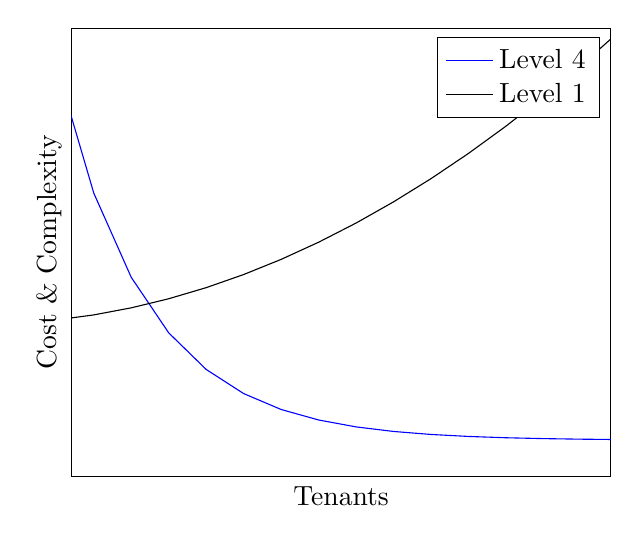
\begin{tikzpicture}
\begin{axis}[
        ymajorticks=false,
    xmajorticks=false,
    xlabel={Tenants},
    ylabel={Cost \& Complexity},
    ymajorgrids=false,
    xmin=-4, xmax=2,
    grid style=dashed,
]
 
\addplot[color=blue]{exp(-x)};
	
	\addplot[color=black] {0.5(x+5)^2 + 20	};
	
\legend{Level 4, Level 1}
\end{axis}
\end{tikzpicture}

\caption{Implementation complexity per tenant}
\label{fig:imp_complexity}
\end{figure}






SaaS maturity level 4 is, however, the archetypal ideal maturity level to execute, but because of its complexity is not always the first multi-tenant level developed by service providers (SP). The 3rd maturity level is also multi-tenant enabled, but does not allow for scaling and therefore inherently contains some risks associated with it such as single point of failure and application instability. Since all tenants share this common instance, the impact of these risks are also (much higher) than with single-tenant applications and should therefore be kept in mind during application design.

\section{Challenges and Requirements of Implementing Multi-tenancy}

Multi-tenancy introduces many common challenges and requirements that need to be addressed in order to be implemented effectively. Common challenges include \cite{Betts2012-ad}:

\begin{itemize}
\item Partitioning
\item Extensibility
\item Provisioning
\item Testability
\item Customization
\item Third Party Components
\item Tenant isolation
\item Security
\end{itemize}

Betts \cite{Betts2012-ad} additionally outlines some of the common requirements a multi-tenant solution should consider and address from the tenant's perspective (see table \ref{table:tenant-requirements}).


These requirements are very important to recognize as they can influence a SP choice of whether or not to design their application to be multi-tenant enabled. For example SP that do not require the scalability and availability, but high levels of security and regulatory compliance might rather implement a single-tenant application that physically isolates its tenant's data.


\section{Conclusion}

This chapter took an overall look at multi-tenancy as an alternative architectural principle used for developing effective SaaS services that utilize many of the advanced capabilities offered by cloud computing. Furthermore, the different levels of SaaS maturity are discussed in relation to multi-tenancy and highlights how fundamental multi-tenancy is to developing good SaaS application. Finally, the economic impact of multi-tenancy is discussed as driving force behind the choice for it to be implemented. The next chapter introduces us to the methodology used in this paper and examines the specifics of how our research problem will be tackled. 
